\documentclass[11pt,a4paper]{article}

% ------------------------------------------------------------
% Paquetes
% ------------------------------------------------------------
\usepackage[utf8]{inputenc}
\usepackage[T1]{fontenc}
\usepackage{lmodern}
\usepackage{microtype}
\usepackage[spanish,es-noindentfirst]{babel}
\usepackage[margin=2.5cm]{geometry}
\usepackage{graphicx}
\usepackage{xcolor}
\usepackage{booktabs}
\usepackage{siunitx}
\usepackage{amsmath}
\usepackage{caption}
\usepackage[colorlinks=true,linkcolor=blue!50!black,citecolor=blue!50!black,urlcolor=blue!50!black]{hyperref}
\usepackage[round]{natbib}

\graphicspath{{figures/}}
\sisetup{output-decimal-marker={,}}

% Resultados numericos generados automaticamente por src/run_pipeline.py
% Archivo generado automaticamente por src/run_pipeline.py. No editar a mano.
\newcommand{\DatasetCityCount}{100}
\newcommand{\DatasetRowCount}{228.175}
\newcommand{\AnalysisStartYear}{1851}
\newcommand{\AnalysisEndYear}{2013}
\newcommand{\BogotaObsCount}{1.952}
\newcommand{\BogotaMean}{20.01}
\newcommand{\BogotaStd}{0.73}
\newcommand{\BogotaMin}{17.93}
\newcommand{\BogotaMax}{22.51}
\newcommand{\ResidStd}{0.315}
\newcommand{\ResidMin}{-1.285}
\newcommand{\ResidMax}{1.180}
\newcommand{\AdfStatistic}{-3.89}
\newcommand{\AdfPValue}{0.0021}
\newcommand{\SarimaOrder}{(1,0,2)}
\newcommand{\SarimaSeasonalOrder}{(0,1,1,12)}
\newcommand{\BacktestRmse}{0.401}
\newcommand{\BacktestMae}{0.334}
\newcommand{\TestSizeMonths}{24}
\newcommand{\FutureHorizonMonths}{24}
\newcommand{\ForecastMeanEnd}{21.39}


% ------------------------------------------------------------
% Portada
% ------------------------------------------------------------
\title{Análisis, Descomposición y Pronóstico de la Serie de Temperatura Mensual de Bogotá (\AnalysisStartYear{}--\AnalysisEndYear{})}
\author{Juan Nicolás Patiño Rodríguez \\ \small Maestría en Inteligencia Artificial y Ciencia de Datos \\ \small Universidad de La Sabana}
\date{\today}

\begin{document}

\maketitle

\begin{abstract}
Se analiza el histórico de temperatura superficial promedio mensual para \DatasetCityCount{} ciudades del mundo, con foco en Bogotá, Colombia, entre \AnalysisStartYear{} y \AnalysisEndYear{}. Tras un análisis gráfico exploratorio y comparativo con ciudades de climas distintos, se aplica una descomposición aditiva de la serie de tiempo y se ajusta un modelo SARIMA para pronosticar su comportamiento futuro. El modelo seleccionado (SARIMA\SarimaOrder{}\,$\times$\,\SarimaSeasonalOrder{}$_{12}$) alcanza un error de \SI{\BacktestRmse}{\celsius} (RMSE) en un conjunto de prueba de \TestSizeMonths{} meses, y se emplea para proyectar la temperatura de Bogotá \FutureHorizonMonths{} meses hacia adelante.
\end{abstract}

\section{Introducción}
\label{sec:introduccion}

% TODO: contexto del problema, objetivo del informe, fuente de datos.

\section{Datos y Metodología}
\label{sec:datos-metodologia}

\subsection{Fuente y estructura de los datos}

El conjunto de datos utilizado (\texttt{Actividad\_2\_Data.csv}) se deriva del histórico
global de temperatura superficial compilado por \citet{berkeleyearth}. Cada registro
corresponde a la temperatura promedio mensual observada en una ciudad, con las siguientes
columnas: \texttt{dt} (fecha, primer día del mes), \texttt{Average\-Temperature} (temperatura
promedio en grados Celsius), \texttt{AverageTemperatureUncertainty} (incertidumbre de la
medición), \texttt{City}, \texttt{Country}, \texttt{Latitude} y \texttt{Longitude}. El
archivo cubre \DatasetCityCount{} ciudades entre 1743 y 2013.

\subsection{Limpieza de datos}

Del total de registros originales, se descartaron aquellos sin temperatura observada
(\texttt{Average\-Temperature} nulo), producto de vacíos en el proceso de medición histórica.
Tras esta depuración quedaron \DatasetRowCount{} registros válidos distribuidos entre las
\DatasetCityCount{} ciudades. Las fechas se tipificaron como \texttt{datetime} y, para cada
ciudad, los registros se ordenaron cronológicamente antes de cualquier análisis posterior.

\subsection{Ventana de análisis para Bogotá}

Al reindexar la serie de Bogotá a una frecuencia mensual regular se identificó un
\textbf{vacío continuo de 20 años} (enero de 1830 a junio de 1850, 246 meses consecutivos sin
registro), además de un puñado de meses aislados sin dato en otros periodos. Rellenar un
vacío de esa magnitud mediante interpolación habría implicado \emph{fabricar} dos décadas de
tendencia y estacionalidad inexistentes en los datos, en lugar de simplemente completar
huecos puntuales. Por esta razón, el análisis y el modelado se restringen al periodo
continuo y confiable de la serie: \textbf{\AnalysisStartYear{}--\AnalysisEndYear{}}, que
comprende \BogotaObsCount{} observaciones mensuales sin vacíos relevantes. Los pocos meses
aislados sin registro dentro de esta ventana sí se completan mediante interpolación lineal
en el tiempo, una operación razonable cuando el hueco es de uno o dos meses.

\subsection{Metodología}

\paragraph{Análisis gráfico.} Se grafica la serie histórica completa de Bogotá y se compara
su perfil climático promedio mes a mes contra ciudades representativas de climas distintos
(templado boreal, desértico/subtropical, tropical monzónico y templado del hemisferio sur),
independientemente del rango de años disponible en cada una. Adicionalmente, se construye un
boxplot mensual para inspeccionar la dispersión y detectar valores atípicos por mes.

\paragraph{Descomposición.} Se aplica una descomposición clásica de tipo aditivo
($Y_t = T_t + S_t + R_t$) con periodo estacional de 12 meses, mediante la función
\texttt{seasonal\_decompose} de la librería \texttt{statsmodels}
\citep{seabold2010statsmodels}. Se opta por el modelo aditivo en lugar del multiplicativo
porque la amplitud del ciclo estacional de temperatura no muestra una relación proporcional
clara con el nivel de la serie.

\paragraph{Modelado y pronóstico.} Se divide la serie en un conjunto de entrenamiento y uno
de prueba, reservando los últimos \TestSizeMonths{} meses para validación. Sobre el conjunto
de entrenamiento se aplica la prueba de Dickey-Fuller aumentada (ADF)
\citep{dickeyfuller1979} para evaluar estacionariedad, y se inspeccionan las funciones de
autocorrelación (ACF) y autocorrelación parcial (PACF) como insumo para acotar el orden del
modelo. El orden final $(p,d,q)\times(P,D,Q)_{12}$ de un modelo SARIMA se selecciona mediante
una búsqueda en grilla que minimiza el criterio de información de Akaike (AIC), ajustando los
modelos con \texttt{SARIMAX} de \texttt{statsmodels}. El modelo seleccionado se evalúa sobre
el conjunto de prueba mediante el error cuadrático medio (RMSE) y el error absoluto medio
(MAE); posteriormente se reajusta sobre la serie completa para proyectar
\FutureHorizonMonths{} meses hacia el futuro, junto con su intervalo de confianza del 95\,\%.

\subsection{Herramientas y reproducibilidad}

Todo el análisis se implementó en Python con tipado estático estricto (verificado con
\texttt{mypy --strict}), utilizando \texttt{pandas} \citep{mckinney2010pandas},
\texttt{statsmodels} \citep{seabold2010statsmodels}, \texttt{scikit-learn} y
\texttt{matplotlib}. Un único script (\texttt{src/run\_pipeline.py}) ejecuta de punta a punta
la carga y limpieza de datos, el análisis gráfico, la descomposición y el modelado,
regenerando de forma determinística tanto las figuras como los valores numéricos citados en
este informe.

\section{Análisis Gráfico}
\label{sec:analisis-grafico}

\subsection{Serie histórica de Bogotá}

La Figura~\ref{fig:serie-historica} muestra la temperatura promedio mensual de Bogotá para
el periodo de análisis \AnalysisStartYear{}--\AnalysisEndYear{}. La serie oscila dentro de una
banda relativamente angosta: su media es de \num{\BogotaMean}\,°C, con una desviación estándar
de apenas \num{\BogotaStd}\,°C y un rango entre \num{\BogotaMin}\,°C y \num{\BogotaMax}\,°C. A
simple vista se aprecia un ligero desplazamiento hacia valores más cálidos en las últimas
décadas del registro, algo que se caracteriza formalmente en la Sección~\ref{sec:descomposicion}.

\begin{figure}[htbp]
  \centering
  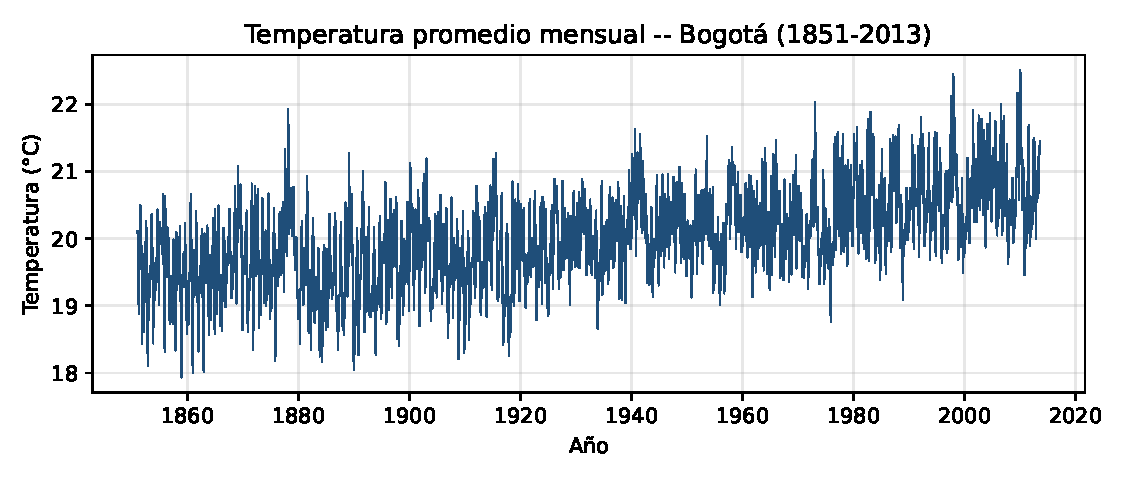
\includegraphics[width=0.85\textwidth]{fig01_serie_historica_bogota.pdf}
  \caption{Temperatura promedio mensual de Bogotá, \AnalysisStartYear{}--\AnalysisEndYear{}.}
  \label{fig:serie-historica}
\end{figure}

\subsection{Comparación climática entre ciudades}

Para contextualizar el comportamiento de Bogotá, la Figura~\ref{fig:perfiles-climaticos}
compara su perfil climático promedio mes a mes contra cuatro ciudades de climas
marcadamente distintos: Berlín (templado boreal, hemisferio norte), El Cairo
(desértico/subtropical), Bangkok (tropical monzónico) y Ciudad del Cabo (templado,
hemisferio sur). El contraste es notable: Berlín y El Cairo muestran una amplitud estacional
de más de \SI{15}{\celsius} entre su mes más frío y más cálido, con el pico de calor a mitad
de año (verano boreal); Ciudad del Cabo exhibe el patrón inverso, con su pico en
enero (verano austral); Bangkok, pese a ser tropical, aún presenta una variación apreciable
asociada al régimen de monzones. \textbf{Bogotá, en cambio, es prácticamente plana a lo
largo del año}, oscilando en un rango menor a \SI{1}{\celsius} entre sus meses extremos. Este
comportamiento es característico de las ciudades ecuatoriales de altura: al estar cerca del
ecuador, la duración del día y el ángulo de incidencia solar varían poco durante el año, por
lo que la temperatura responde más a la altitud (Bogotá se ubica a más de \SI{2600}{\metre}
sobre el nivel del mar) que a un ciclo estacional térmico marcado.

\begin{figure}[htbp]
  \centering
  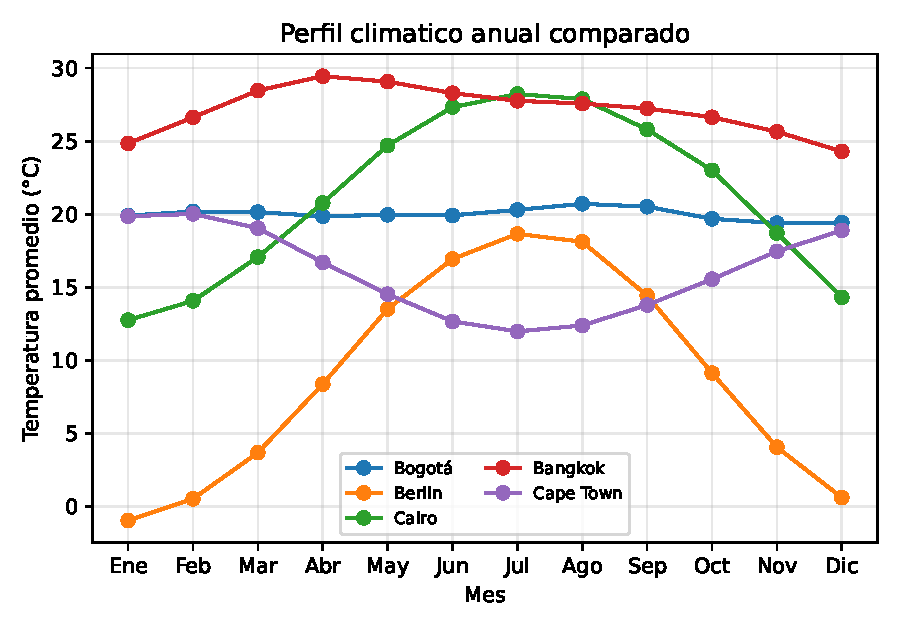
\includegraphics[width=0.75\textwidth]{fig02_perfiles_climaticos.pdf}
  \caption{Perfil climático anual promedio (temperatura media por mes) para cinco ciudades
    de climas distintos.}
  \label{fig:perfiles-climaticos}
\end{figure}

\subsection{Distribución mensual y valores atípicos}

La Figura~\ref{fig:boxplot-mensual} presenta un boxplot mes a mes de la temperatura de
Bogotá. Consistente con la baja amplitud estacional observada, las medianas mensuales son
muy similares entre sí, y los rangos intercuartílicos son estrechos. Se observan algunos
valores atípicos, tanto por encima como por debajo de los bigotes, distribuidos a lo largo
de varios meses; estos son compatibles con anomalías climáticas interanuales (p. ej. eventos
El Niño/La Niña), más que con un patrón estacional adicional no capturado por el ciclo de 12
meses.

\begin{figure}[htbp]
  \centering
  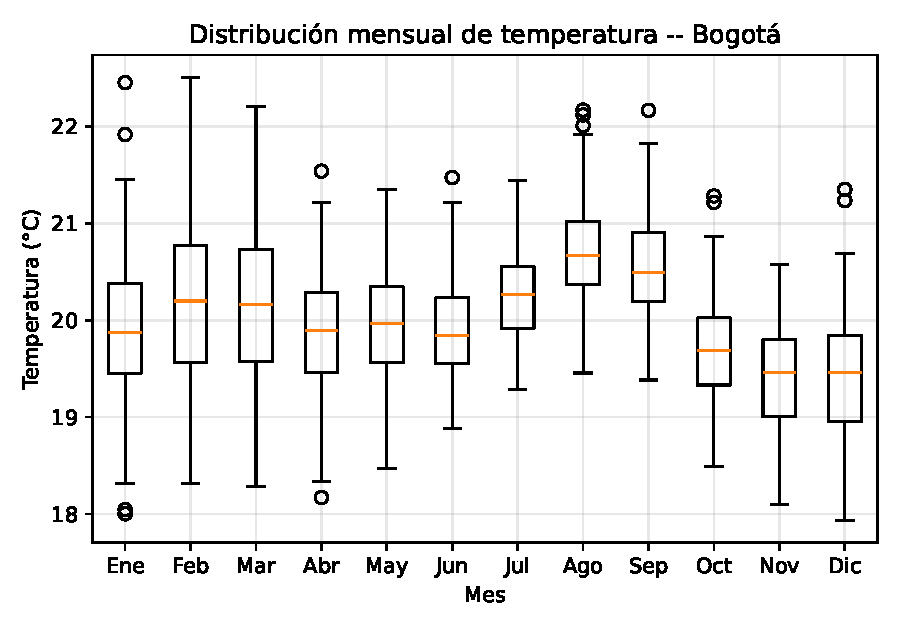
\includegraphics[width=0.75\textwidth]{fig03_boxplot_mensual_bogota.pdf}
  \caption{Distribución de la temperatura mensual de Bogotá por mes calendario.}
  \label{fig:boxplot-mensual}
\end{figure}

\section{Descomposición de la Serie de Tiempo}
\label{sec:descomposicion}

% TODO: metodologia de seasonal_decompose, interpretacion de tendencia,
% estacionalidad y residuos.

\section{Modelado y Pronóstico}
\label{sec:modelado-pronostico}

% TODO: split train/test, prueba ADF, ACF/PACF, seleccion de orden SARIMA,
% pronostico con intervalos de confianza.

\section{Resultados y Discusión}
\label{sec:resultados-discusion}

% TODO: evaluacion critica de calidad/limitaciones del pronostico, metricas,
% relacion con la descomposicion.

\section{Conclusiones}
\label{sec:conclusiones}

% TODO: hallazgos clave y limitaciones del estudio.


\bibliographystyle{apalike}
\bibliography{references}

\end{document}
